\section{Methodology}\label{sec:methodology}
\subsection{Data and preprocessing}\label{sec:data}
\subsubsection{Price data and realized volatility}
We construct realized volatility from cryptocurrency price data sampled at
15-minute intervals. For Bitcoin, we use BTC/USD candles from Bitstamp,
resampled from the supplied one-minute observations. For Ethereum, we use
ETH/USDT candles resampled from five-minute observations. Duplicate raw
timestamps are removed, keeping the last observation, and bars without a
closing price are dropped. After feature construction and alignment with
the news sample, the usable histories begin in January 2017 for Bitcoin
and January 2018 for Ethereum. The out-of-sample analysis covers six
half-year test periods from January 2023 through December 2025.

At each bar $t$, the intraday log return is
\begin{equation}
 r_t=\log P_t^{\mathrm{close}}-\log P_{t-1}^{\mathrm{close}}.
\end{equation}
Following the realized-variance approach of \citet{Andersen2003}, we form
the forward target as a sum of squared returns:
\begin{equation}
 \RV_{t,H}=\sum_{j=1}^{H}r_{t+j}^{2}.\label{eq:rv}
\end{equation}
We target $H=4$ and $H=16$, corresponding to one and four hours on the
15-minute grid. Although we use the conventional term volatility
forecasting, the forecast target is realized \emph{variance}; neither a
square root nor annualization is applied in the loss functions. The
target uses 15-minute close-to-close returns rather than every underlying
one-minute price observation.

Realized variance is heavily right-skewed. We therefore evaluate and train
the neural forecasts using the transformed target
$y_t=\log(\RV_{t,H}+\epsilon)$, with $\epsilon=10^{-10}$. The training
objective is Huber loss on this log scale, described in
Section~\ref{sec:training}. Missing price bars are not interpolated, so
the nominal horizon can span more than $H\times15$ minutes across a gap.
All targets are calculated before the chronological data partitions.

\subsubsection{Time-series features}
From the 15-minute OHLCV bars, we engineer twelve features that capture
multi-scale volatility, return dynamics, and trading activity.
The feature set is motivated by the heterogeneous autoregressive
framework of \citet{Corsi_2008}, in which information at different
aggregation scales contributes to the persistence of realized variance.
Table~\ref{tab:ts_features} summarizes the inputs.

\begin{table}[htbp]
\centering\small
\caption{Time-series input features}\label{tab:ts_features}
\begin{tabular}{@{}lp{9.5cm}@{}}
\toprule
Feature & Description \\
\midrule
$\mathrm{rv}_4,\mathrm{rv}_{16},\mathrm{rv}_{96},\mathrm{rv}_{384}$ & Sum of squared returns over trailing 1h, 4h, 24h, and 4-day windows \\
$\mathrm{log\_ret}$ & Log return of the current bar \\
$\mathrm{mom}_4,\mathrm{mom}_{16}$ & Cumulative log return over the trailing 1h and 4h \\
$\mathrm{hl\_range}_4$ & Trailing 1h mean of $(\mathrm{high}-\mathrm{low})/\mathrm{close}$ \\
$\mathrm{vol\_ratio}_4$ & Current volume divided by the trailing 1h mean volume \\
$\mathrm{skew}_{16},\mathrm{kurt}_{16}$ & Return skewness and excess kurtosis over the trailing 4h \\
$\mathrm{log\_close}$ & Log price level \\
\bottomrule
\end{tabular}
\end{table}

The variance aggregates are neural counterparts to the multi-scale HAR
components, adapted to continuously traded cryptocurrency markets.
Higher-order moments describe return asymmetry and tail behavior
\citep{Patton_2015}, while the volume ratio captures a dimension of
information flow not contained in past returns alone
\citep{ANDERSEN_1996}. Trailing features include the current completed
bar. Each feature is standardized using its mean and sample standard
deviation in the training portion of the expanding window, and the
standardized values are clipped to $[-10,10]$. These normalization
parameters are held fixed during validation and testing.

\subsubsection{News corpus and reactive filtering}
We use CoinDesk news records with article text and UTC publication
timestamps. Before January 2026, the processed corpus contains 25,447
BTC-labelled records and 10,277 ETH-labelled records. These are
asset-specific observations: an article associated with both assets can
appear in both samples. After the recap filter, 19,249 BTC and 8,735 ETH
records remain. The underlying file also contains early-2026 articles;
the publication-time cutoff prevents those later records from entering
any forecast in the 2023--2025 test sample.

A key preprocessing step addresses reactive news contamination:
articles that describe a price movement already in progress rather than
report a new information event. We remove articles carrying the editorial
tags price-news, Markets News, Market Wrap, Bitcoin Price, Technical
Analysis, First Mover, Bitcoin Long \& Short, Crypto Long \& Short,
Markets Daily, Asia Pacific, or Trading. A small title-based augmentation
matches ``market wrap'', Bitcoin/BTC followed by a dollar sign at the
beginning of a headline, and the First Mover Asia/Americas/Europe series.
The filter is deterministic and does not use future returns.

Filtering reduces the direct use of price-recap language, but it is not
a guarantee that every retained article represents an exogenous shock.
An article reporting a market movement can still survive when its tags
and title do not match the rules. This distinction matters for the
interpretation of the case study and category results below.

For each forecast, we retrieve retained articles in the preceding twelve
hours, with publication times strictly earlier than the stored bar
timestamp. The timestamp is the first raw observation in the resampled
bar, generally its left-hand endpoint. Since the price features use the
completed current bar, forecasts are interpreted as end-of-bar forecasts
with this earlier news cutoff. The news age used by the model is measured
from the stored timestamp. These timing conventions are applied
consistently to the main model and its ablations.

\subsubsection{CryptoBERT embeddings}\label{sec:cryptobert}
Each article is represented by a 768-dimensional vector from the
pretrained \texttt{ElKulako/\allowbreak cryptobert} checkpoint
\citep{Kulakowski_2023}. The encoder processes the stored article text,
truncated to at most 512 tokens. We average its final hidden states over
the positions enabled by the attention mask and normalize the resulting
vector to unit Euclidean length. Embeddings are precomputed and held
fixed during volatility-model training.

The main model uses the complete 768-dimensional representation, followed
by a learned LayerNorm at the input to the news head. No PCA is applied
in the primary specification. A 256-dimensional representation is
introduced only in the news-representation ablation, where PCA is fitted
separately on training-period retained articles in each window.
CryptoBERT's cryptocurrency-oriented representation offers a way to
encode event descriptions beyond a fixed sentiment category. Whether
that additional information improves forecasts is an empirical question
addressed in Section~\ref{sec:news_representations}.

\begin{figure}[htbp]
\centering
\begin{adjustbox}{max width=\textwidth}
\begin{tikzpicture}[
 box/.style={draw,rounded corners,align=center,text width=5.1cm,minimum height=1cm,font=\small},
 arr/.style={-{Stealth},thick},node distance=7mm]
\node[box,fill=teal!8] (ts) {12 standardized price features\\MLP: $12\to64\to32\to16\to1$};
\node[box,fill=orange!8,right=9mm of ts] (news) {Frozen CryptoBERT, token mean pooling\\768 dimensions, $L^2$ normalization};
\node[box,fill=teal!8,below=of ts] (base) {Positive baseline $v_t^{\mathrm{TS}}$\\P1: train; P2: freeze weights};
\node[box,fill=orange!8,below=of news] (head) {LayerNorm; MLP $768\to128\to32\to2$\\Per-article $s_k$, $\lambda_k$};
\node[box,fill=orange!8,below=of head] (agg) {Past 12 hours, publication time $<\tau_t$\\$S_t=\sum_k s_k e^{-\lambda_k\Delta t_{tk}}$};
\node[box,fill=violet!8,below=24mm of base,text width=5.1cm] (out) {$\widehat{\RV}_{t,H}=v_t^{\mathrm{TS}} e^{\clip(aS_t+b,-2,2)}$\\P2: train the news correction};
\draw[arr] (ts)--(base);
\draw[arr] (news)--(head);
\draw[arr] (head)--(agg);
\draw[arr] (base)--(out);
\draw[arr] (agg.south)|-(out.east);
\end{tikzpicture}
\end{adjustbox}
\caption{The NED architecture. The first training phase estimates the
time-series baseline; the second freezes its weights and learns the
article-dependent news correction. The final forecast is produced by
the second-phase model selected on validation loss.}
\label{fig:architecture}
\end{figure}

\begin{figure}[htbp]
\centering
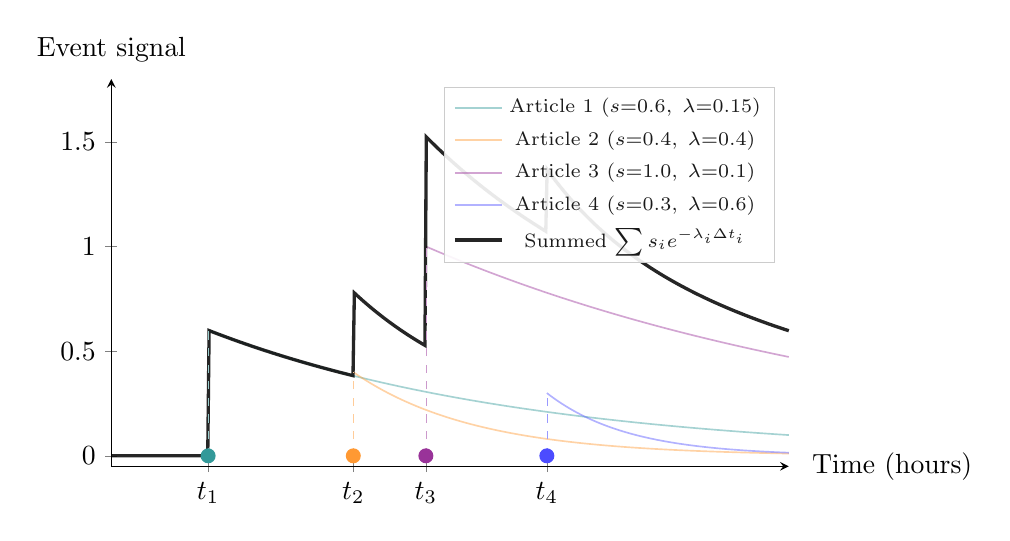
\begin{tikzpicture}
\begin{axis}[
    width=0.84\textwidth,
    height=6.5cm,
    xlabel={Time (hours)},
    ylabel={Event signal},
    xmin=0, xmax=14,
    ymin=-0.05, ymax=1.8,
    xtick={2,5,6.5,9},
    xticklabels={$t_1$, $t_2$, $t_3$, $t_4$},
    ytick={0,0.5,1.0,1.5},
    axis lines=left,
    every axis x label/.style={at={(ticklabel* cs:1.02)}, anchor=west},
    every axis y label/.style={at={(ticklabel* cs:1.02)}, anchor=south},
    legend style={
        at={(0.98,0.98)}, anchor=north east,
        font=\scriptsize, draw=gray!40,
        fill=white, fill opacity=0.9,
        row sep=1pt,
    },
    grid=none,
    clip=false,
]

% --- Individual decay curves (thin, colored) ---
\addplot[domain=2:14, samples=200, teal!70, semithick, opacity=0.5]
    {0.6 * exp(-0.15*(x-2))};
\addlegendentry{Article 1 ($s{=}0.6,\;\lambda{=}0.15$)}

\addplot[domain=5:14, samples=200, orange!70, semithick, opacity=0.5]
    {0.4 * exp(-0.4*(x-5))};
\addlegendentry{Article 2 ($s{=}0.4,\;\lambda{=}0.4$)}

\addplot[domain=6.5:14, samples=200, violet!70, semithick, opacity=0.5]
    {1.0 * exp(-0.1*(x-6.5))};
\addlegendentry{Article 3 ($s{=}1.0,\;\lambda{=}0.1$)}

\addplot[domain=9:14, samples=200, blue!60, semithick, opacity=0.5]
    {0.3 * exp(-0.6*(x-9))};
\addlegendentry{Article 4 ($s{=}0.3,\;\lambda{=}0.6$)}

% --- Summed signal (single expression using boolean conditions) ---
\addplot[domain=0:14, samples=500, black, very thick, opacity=0.85]
    { (x>=2)  * 0.6 * exp(-0.15*(x-2))
    + (x>=5)  * 0.4 * exp(-0.4*(x-5))
    + (x>=6.5)* 1.0 * exp(-0.1*(x-6.5))
    + (x>=9)  * 0.3 * exp(-0.6*(x-9))
    };
\addlegendentry{Summed $\sum s_i e^{-\lambda_i \Delta t_i}$}

% --- Article arrival markers on x-axis ---
\addplot[only marks, mark=*, mark size=2.5pt, teal!80, forget plot] coordinates {(2,0)};
\addplot[only marks, mark=*, mark size=2.5pt, orange!80, forget plot] coordinates {(5,0)};
\addplot[only marks, mark=*, mark size=2.5pt, violet!80, forget plot] coordinates {(6.5,0)};
\addplot[only marks, mark=*, mark size=2.5pt, blue!70, forget plot] coordinates {(9,0)};

% --- Dashed vertical lines at arrivals ---
\draw[teal!40, dashed, very thin] (axis cs:2,0) -- (axis cs:2,0.6);
\draw[orange!40, dashed, very thin] (axis cs:5,0) -- (axis cs:5,0.4);
\draw[violet!40, dashed, very thin] (axis cs:6.5,0) -- (axis cs:6.5,1.0);
\draw[blue!40, dashed, very thin] (axis cs:9,0) -- (axis cs:9,0.3);

\end{axis}
\end{tikzpicture}
\caption{Event signal accumulation. Each article contributes a decaying signal with magnitude $s_k$ and rate $\lambda_k$. The aggregate is the sum of the active article kernels. Curves illustrate the mechanism and are not empirical parameter estimates; the horizontal scale and the displayed rates use hours. The model is inspired by Hawkes-type kernels but does not fit a self-exciting arrival intensity.}
\label{fig:decay_stacking}
\end{figure}


\subsection{NED architecture}\label{sec:architecture}
The News Event Decay model decomposes the log forecast into a
time-series component and a news-driven correction. Let
$v_t^{\mathrm{ts}}>0$ be the time-series variance forecast and $S_t$ the
aggregate article signal. The combination is
\begin{equation}
 \log\widehat{\RV}_{t,H}=\log v_t^{\mathrm{ts}}+
    \clip(aS_t+b,-2,2).\label{eq:residual}
\end{equation}
Thus the residual is additive in log units and multiplicative on variance
levels. The small stabilizer $\epsilon$ is introduced when calculating
the training and evaluation losses, rather than in the architecture's
combination rule. Figure~\ref{fig:architecture} illustrates the two branches.

\subsubsection{Time-series branch}
The time-series branch maps the twelve standardized features to a
positive variance forecast through a feedforward network with widths
$12\to64\to32\to16\to1$. Hidden layers use ReLU activations, the first
hidden layer is followed by dropout with probability 0.2, and the output
uses Softplus. This can be viewed as a nonlinear extension of the
multi-scale HAR representation: variance components enter alongside
return, range, volume, and higher-moment features, allowing their
interactions to be learned rather than imposed linearly.

\subsubsection{News event branch}
Let $e_k\in\mathbb R^{768}$ and $\tau_k$ denote an eligible article's
embedding and publication time. A news MLP with hidden widths 128 and 32
and ReLU activations maps its normalized embedding to two raw outputs:
\begin{align}
 (u_k,v_k)&=g_\psi(\operatorname{LayerNorm}(e_k)),\\
 s_k&=\softplus(u_k),\qquad
 \lambda_k=0.001+0.499\sigmoid(v_k).\label{eq:impact_head}
\end{align}
The magnitude $s_k$ is positive, while $\lambda_k$ lies between 0.001
and 0.5 per minute. For an article age
$\Delta t_k=(\tau_t-\tau_k)/60$ in minutes, the event signal is
\begin{equation}
 S_t=\sum_{k\in\mathcal N_t}s_k\exp(-\lambda_k\Delta t_k),
 \qquad\mathcal N_t=\{k:\tau_t-12\mathrm{h}\leq\tau_k<\tau_t\}.
 \label{eq:decay}
\end{equation}
Only retained articles enter $\mathcal N_t$. Padding is masked out, and
the sum is not divided by the number of articles.

The architecture is inspired by the event-kernel structure of Hawkes
processes \citep{HAWKES1971}. Here the arrival times are observed news
timestamps, and both kernel parameters depend on article content; no
arrival-intensity likelihood or self-excitation parameter is estimated.
The exponential half-life is $h_{1/2,k}=\log(2)/\lambda_k$, bounded
approximately between 1.39 and 693 minutes. The twelve-hour lookback
truncates a contribution regardless of its untruncated half-life.
Figure~\ref{fig:decay_stacking} illustrates how article signals accumulate.

\subsubsection{Residual combination}
The variance forecast corresponding to Equation~\eqref{eq:residual} is
\begin{equation}
 \widehat{\RV}_{t,H}=v_t^{\mathrm{ts}}
      \exp\!\left[\clip(aS_t+b,-2,2)\right].
\end{equation}
The residual weight $a$ and intercept $b$ are initialized to zero,
so that the news branch begins with the unadjusted time-series forecast.
Clipping bounds the adjustment factor between $e^{-2}$ and $e^2$.
The additional time-series scale parameter remains fixed at one.

This structure makes the role of the news signal explicit. Away from
clipping, article $k$ contributes $a s_k e^{-\lambda_k\Delta t_k}$ to the
log correction. The shared loading can be positive or negative, and the
intercept permits baseline recalibration even when no news is present.
Consequently a positive $s_k$ does not itself identify a positive causal
variance shock. The benefit of the decomposition is that it separates
article timing and persistence from the final calibration of the forecast.

\subsection{Training procedure}\label{sec:training}
Training proceeds in two sequential phases. P1 estimates the time-series
branch; P2 holds those weights fixed while fitting the news correction.
Both phases minimize Huber loss on the log variance error,
\begin{align}
 e_t&=\log(\widehat{\RV}_{t,H}+\epsilon)-\log(\RV_{t,H}+\epsilon),\\
 \mathcal L&=\frac1N\sum_t\rho_{0.5}(e_t),\qquad
 \rho_\delta(e)=\begin{cases}\frac12e^2,&|e|\leq\delta,\\
 \delta(|e|-\frac12\delta),&|e|>\delta.
 \end{cases}\label{eq:loss}
\end{align}
The objective downweights large log errors relative to squared loss.
It is distinct from both log-MSE and QLIKE, the forecast losses used
for evaluation. The staged design directs the news branch toward errors
remaining after the time-series fit, while preserving the P1 model as
an exact no-news comparator.

\begin{table}[htbp]
\centering\small
\caption{Training phase configuration}\label{tab:training_phases}
\begin{tabular}{@{}lcc@{}}
\toprule
 & Phase 1 & Phase 2 \\
\midrule
TS weights & Trained & Frozen \\
News branch & Frozen & Trained \\
Learning rate & $10^{-4}$ & $5\times10^{-5}$ \\
Maximum epochs & 100 & 120 \\
Early-stopping patience & 15 & 20 \\
Batch size & 64 & 64 \\
Main-model auxiliary loss & Disabled & Disabled \\
\bottomrule
\end{tabular}
\end{table}

We use AdamW \citep{adamw} with weight decay 0.01. P2 gradients are
clipped at norm 1.0, and the selected model is the P2 checkpoint with
the lowest primary validation loss. No joint fine-tuning follows P2.
Initialization/P1 use seed 7 and P2 uses seed 42. The time-series dropout
remains active during P2 training despite its frozen weights; evaluation
disables dropout. The auxiliary loss of the main model is zero.

\subsubsection{Expanding window evaluation}
Each model is trained on all observations before a six-month validation
period and evaluated on the subsequent half-year. The training history
expands monotonically, and model selection uses validation loss only.
The six test periods begin in January 2023, July 2023, January 2024,
July 2024, January 2025, and July 2025. The total test sample is 104,570
BTC bars and 104,641 ETH bars at each horizon.

Two implementation conventions qualify this chronological design.
Validation and test upper bounds include 00:00 UTC on their final date,
omitting the remaining bars on that date. Training labels are not purged
when their forward returns extend across the start of validation.
These conventions are held fixed across comparisons; sensitivity to
an embargo and full end-of-day bounds remains a limitation of the
experimental design. The ablations reuse each window's selected P1
state and retrain the alternative P2 branches on the same partitions.

\subsection{Baselines}\label{sec:baselines}
We compare NED with four benchmarks spanning parametric and neural
time-series forecasting, including a parametric model augmented with
the same article-level decay mechanism.

\subsubsection{HAR}
The adapted HAR model \citep{Corsi_2008} forecasts log realized variance
from four trailing variance components:
\begin{equation}
 \hat y_t^{\mathrm{HAR}}=\beta_0+\beta_1\mathrm{rv}_4+
 \beta_2\mathrm{rv}_{16}+\beta_3\mathrm{rv}_{96}+\beta_4\mathrm{rv}_{384}.
 \label{eq:har}
\end{equation}
Coefficients are estimated by ordinary least squares on the training
set, and forecasts are exponentiated without a lognormal bias
correction. The regressors are variance levels, not their logarithms.
HAR uses four features whereas the neural time-series branch uses
twelve, so their comparison changes both flexibility and the feature set.

\subsubsection{EGARCH}
The EGARCH model of \citet{Nelson_1991} accommodates asymmetric responses
of conditional variance to return innovations. We estimate an
EGARCH(1,1) with one asymmetric term, a zero mean, and Student-$t$
innovations on training-period 15-minute returns multiplied by 100.
Parameters are then fixed while the conditional variance recursion is
filtered forward. The benchmark scales the filtered one-bar variance
by the forecast horizon:
\begin{equation}
 v_{t,H}^{\mathrm{EGARCH}}=H\hat\sigma_t^2,\label{eq:egarch}
\end{equation}
after undoing the return scaling. This horizon-scaled filtered variance
is the comparator evaluated here; it is not an iterated sum of future
conditional variance forecasts.

\subsubsection{EGARCH+NED}
The hybrid replaces the neural time-series forecast with the EGARCH
baseline while preserving the multiplicative news correction:
\begin{equation}
 \widehat{\RV}_{t,H}^{\mathrm{EGARCH+NED}}=
 v_{t,H}^{\mathrm{EGARCH}}e^{\clip(aS_t+b,-2,2)}.\label{eq:egarch_ned}
\end{equation}
A separate article network is trained against the fixed EGARCH
baseline with learning rate $2\times10^{-4}$, a 120-epoch cap,
patience 20, and gradient clipping at 1.0. The primary objective is
Huber-on-log loss. In this hybrid, a news-only auxiliary prediction
head adds a loss with weight 0.1, while validation selects primary
forecast loss. Thus this comparison also includes a difference in
auxiliary training from the main model, whose auxiliary loss is disabled.

\subsubsection{TS-only}
TS-only is the selected P1 time-series branch, evaluated without the
news correction. It uses precisely the same time-series weights,
features, normalization, and initial training run as NED. The
NED--TS-only comparison therefore measures the incremental contribution
of the complete P2 correction, including its intercept, rather than
differences between separately trained baseline networks.

\subsection{Evaluation metrics and statistical tests}\label{sec:metrics}
We compute all metrics within each test window and report their
arithmetic means across the six windows. This avoids the change in
the $R^2$ reference variance that would occur when pooling distinct
volatility regimes. Per-window results appear in the appendix.

\subsubsection{Coefficient of determination}
The coefficient of determination uses log realized variance:
\begin{equation}
 R_w^2=1-\frac{\sum_{t\in w}(y_t-\hat y_t)^2}
                   {\sum_{t\in w}(y_t-\bar y_w)^2},\label{eq:r2}
\end{equation}
where $\bar y_w$ is the mean of actual log variance in the test window.
Negative values indicate worse performance than that ex-post constant
mean. It is not a comparison with the training-sample mean forecast.

\subsubsection{Directional accuracy}
We retain the label DA used in the experiment, whose definition is
accuracy relative to a common volatility threshold:
\begin{equation}
 \mathrm{DA}_w=\frac1{N_w}\sum_{t\in w}\mathbf1\!
 \left\{\mathbf1(\RV_{t,H}>m_w)=
          \mathbf1(\widehat{\RV}_{t,H}>m_w)\right\},\label{eq:da}
\end{equation}
where $m_w$ is the median actual variance in the test window. This
measures agreement about high versus low variance, not agreement about
successive increases or decreases. The median is an ex-post threshold.

\subsubsection{QLIKE}
The QLIKE loss is
\begin{equation}
 \mathrm{QLIKE}_w=\frac1{N_w}\sum_{t\in w}(q_t-\log q_t-1),\quad
 q_t=\frac{\RV_{t,H}+\epsilon}{\widehat{\RV}_{t,H}+\epsilon}.
 \label{eq:qlike}
\end{equation}
QLIKE is sensitive to underprediction of large realized variances and
provides a different ranking criterion from log-MSE. Its use with
noisy volatility proxies is motivated by \citet{Patton_2011}.

\subsubsection{Mean squared error}
MSE is computed in log units:
\begin{equation}
 \mathrm{MSE}_w=\frac1{N_w}\sum_{t\in w}(y_t-\hat y_t)^2.\label{eq:mse}
\end{equation}
It weights proportional errors more evenly across variance levels
than level-MSE and remains distinct from the robust training objective.

\subsubsection{Diebold-Mariano test with small-sample correction}
For the inference reported in the tables, we apply the loss-differential
test of \citet{DM_1995} with the finite-sample correction of
\citet{Harvey_1997}. With $d_t=L_t^{\mathrm{NED}}-L_t^{\mathrm{TS}}$,
the statistic is
\begin{equation}
 \mathrm{DM}^{*}=\sqrt{\frac{N+1-2H+H(H-1)/N}{N}}
       \frac{\bar d}{\sqrt{\widehat\Omega/N}}.\label{eq:dm}
\end{equation}
We estimate $\widehat\Omega$ using Bartlett weights through lag
$H-1$ and report two-sided Student-$t$ probabilities with $N-1$
degrees of freedom. Negative statistics favor NED. The tests are
recomputed from the saved observation-level forecasts for this paper.
Uncorrected normal-reference tests with bandwidth $H$, produced by
the main training pipeline, are retained as a sensitivity check; the
aggregate conclusions are unchanged.

Aggregate tests concatenate chronological loss differentials from
the six test windows. They therefore weight observations, whereas
summary metrics weight windows equally. Lag pairs crossing the joins
are retained. Reported probabilities are unadjusted for multiple
comparisons and do not capture variation across independent training
seeds. Statistical significance is interpreted together with the
per-window pattern and the size of the forecast improvement.
